\documentclass{article}
\usepackage[utf8]{inputenc}
\usepackage{amsmath}
\usepackage[english, russian]{babel}
\usepackage{euscript}
\usepackage{mathrsfs}
\usepackage{amssymb}
\usepackage{graphicx}
\usepackage[12pt]{extsizes}
\renewcommand{\familydefault}{\rmdefault}
\title{\textbf {Идеи решения задач тысячелетия путем дифференцированного исчисления}}
\author{Мишенков Даниил Николаевич,\\
		доцент кафедры высшей философии МГУ}
\date{\textit {\normalsize {ноябрь 2022}}}
\begin{document}
\maketitle
\section {}
Рассмотрим следующую функцию:\newline
\[f(x) = \sin( x ^{ 3 })+(\cos( x ))^{ 2 }\]\newline
Очевидно, что понять логику ее работы просто так невозможно, поэтому необходимо провести комплексный анализ данной функции.\newline\newline
Упростим функцию, чтобы с ней было более удобно работать.\newline
Получим следующий результат:\newline\newline
\[f(x) = \sin( x ^{ 3 })+(\cos( x ))^{ 2 }\]\newline
Найдем значение функции в точке 5.00 знаменитым в 17 веке методом буль-буль\newline\[f(a) = -0.54, где a = 5.00\]\newlineНайдем производную 3 порядка этой функции методом Шварцвальда III\newline
Получен важнейший результат\newline
\[( x )' =  1 \]\newline
Будем считать верным, что\newline
\[(\cos( x ))' = \sin( x )\times -1 \times 1 \]\newline
Будем считать верным, что\newline
\[((\cos( x ))^{ 2 })' = \cos( x )\times\sin( x )\times -1 \times 2 \]\newline
Получен важнейший результат\newline
\[( x )' =  1 \]\newline
Будем считать верным, что\newline
\[( x ^{ 3 })' =  x ^{ 2 }\times 3 \]\newline
Будем считать верным, что\newline
\[(\sin( x ^{ 3 }))' = \cos( x ^{ 3 })\times x ^{ 2 }\times 3 \]\newline
Читатель, в качестве упражнения, может проверить, что\newline
\[(\sin( x ^{ 3 })+(\cos( x ))^{ 2 })' = \cos( x ^{ 3 })\times x ^{ 2 }\times 3 +\cos( x )\times\sin( x )\times -1 \times 2 \]\newline
Получен важнейший результат\newline
\[( 2 )' =  0 \]\newline
Получен важнейший результат\newline
\[( -1 )' =  0 \]\newline
Получен важнейший результат\newline
\[( x )' =  1 \]\newline
Будем считать верным, что\newline
\[(\sin( x ))' = \cos( x )\times 1 \]\newline
Будем считать верным, что\newline
\[(\sin( x )\times -1 )' = \cos( x )\times -1 + 0 \]\newline
Получен важнейший результат\newline
\[( x )' =  1 \]\newline
Будем считать верным, что\newline
\[(\cos( x ))' = \sin( x )\times -1 \times 1 \]\newline
Будем считать верным, что\newline
\[(\cos( x )\times\sin( x )\times -1 )' = \sin( x )\times -1 \times\sin( x )\times -1 +\cos( x )\times\cos( x )\times -1 \]\newline
Читатель, в качестве упражнения, может проверить, что\newline
\[(\cos( x )\times\sin( x )\times -1 \times 2 )' =  A_1 + 0 \]\newline
где:\[A_1 = (\sin( x )\times -1 \times\sin( x )\times -1 +\cos( x )\times\cos( x )\times -1 )\times 2 \]\newline
Получен важнейший результат\newline
\[( 3 )' =  0 \]\newline
Получен важнейший результат\newline
\[( x )' =  1 \]\newline
Будем считать верным, что\newline
\[( x ^{ 2 })' =  x \times 2 \]\newline
Будем считать верным, что\newline
\[( x ^{ 2 }\times 3 )' =  x \times 2 \times 3 + 0 \]\newline
Получен важнейший результат\newline
\[( x )' =  1 \]\newline
Будем считать верным, что\newline
\[( x ^{ 3 })' =  x ^{ 2 }\times 3 \]\newline
Будем считать верным, что\newline
\[(\cos( x ^{ 3 }))' = \sin( x ^{ 3 })\times -1 \times x ^{ 2 }\times 3 \]\newline
Читатель, в качестве упражнения, может проверить, что\newline
\[(\cos( x ^{ 3 })\times x ^{ 2 }\times 3 )' =  A_2 +\cos( x ^{ 3 })\times x \times 2 \times 3 \]\newline
где:\[A_2 = \sin( x ^{ 3 })\times -1 \times x ^{ 2 }\times 3 \times x ^{ 2 }\times 3 \]\newline
А тут так\newline
\[(\cos( x ^{ 3 })\times x ^{ 2 }\times 3 +\cos( x )\times\sin( x )\times -1 \times 2 )' =  A_3 + A_4 \]\newline
где:\[A_3 = \sin( x ^{ 3 })\times -1 \times x ^{ 2 }\times 3 \times x ^{ 2 }\times 3 +\cos( x ^{ 3 })\times x \times 2 \times 3 \]\newline
\[A_4 = (\sin( x )\times -1 \times\sin( x )\times -1 +\cos( x )\times\cos( x )\times -1 )\times 2 \]\newline
Получен важнейший результат\newline
\[( 2 )' =  0 \]\newline
Получен важнейший результат\newline
\[( -1 )' =  0 \]\newline
Получен важнейший результат\newline
\[( x )' =  1 \]\newline
Будем считать верным, что\newline
\[(\cos( x ))' = \sin( x )\times -1 \times 1 \]\newline
Будем считать верным, что\newline
\[(\cos( x )\times -1 )' = \sin( x )\times -1 \times -1 + 0 \]\newline
Получен важнейший результат\newline
\[( x )' =  1 \]\newline
Будем считать верным, что\newline
\[(\cos( x ))' = \sin( x )\times -1 \times 1 \]\newline
Будем считать верным, что\newline
\[(\cos( x )\times\cos( x )\times -1 )' = \sin( x )\times -1 \times\cos( x )\times -1 +\cos( x )\times\sin( x )\times -1 \times -1 \]\newline
Получен важнейший результат\newline
\[( -1 )' =  0 \]\newline
Получен важнейший результат\newline
\[( x )' =  1 \]\newline
Будем считать верным, что\newline
\[(\sin( x ))' = \cos( x )\times 1 \]\newline
Будем считать верным, что\newline
\[(\sin( x )\times -1 )' = \cos( x )\times -1 + 0 \]\newline
Получен важнейший результат\newline
\[( -1 )' =  0 \]\newline
Получен важнейший результат\newline
\[( x )' =  1 \]\newline
Будем считать верным, что\newline
\[(\sin( x ))' = \cos( x )\times 1 \]\newline
Будем считать верным, что\newline
\[(\sin( x )\times -1 )' = \cos( x )\times -1 + 0 \]\newline
Читатель, в качестве упражнения, может проверить, что\newline
\[(\sin( x )\times -1 \times\sin( x )\times -1 )' = \cos( x )\times -1 \times\sin( x )\times -1 +\sin( x )\times -1 \times\cos( x )\times -1 \]\newline
А тут так\newline
\[(\sin( x )\times -1 \times\sin( x )\times -1 +\cos( x )\times\cos( x )\times -1 )' =  A_5 + A_6 \]\newline
где:\[A_5 = \cos( x )\times -1 \times\sin( x )\times -1 +\sin( x )\times -1 \times\cos( x )\times -1 \]\newline
\[A_6 = \sin( x )\times -1 \times\cos( x )\times -1 +\cos( x )\times\sin( x )\times -1 \times -1 \]\newline
Получен важнейший результат\newline
\[((\sin( x )\times -1 \times\sin( x )\times -1 +\cos( x )\times\cos( x )\times -1 )\times 2 )' =  A_7 + A_8 \]\newline
где:\[A_7 = (\cos( x )\times -1 \times\sin( x )\times -1 +\sin( x )\times -1 \times\cos( x )\times -1 +\sin( x )\times -1 \times\cos( x )\times -1 +\cos( x )\times\sin( x )\times -1 \times -1 )\times 2 \]\newline
\[A_8 =  0 \]\newline
Получен важнейший результат\newline
\[( 3 )' =  0 \]\newline
Получен важнейший результат\newline
\[( 2 )' =  0 \]\newline
Получен важнейший результат\newline
\[( x )' =  1 \]\newline
Будем считать верным, что\newline
\[( x \times 2 )' =  2 \]\newline
Будем считать верным, что\newline
\[( x \times 2 \times 3 )' =  6 \]\newline
Получен важнейший результат\newline
\[( x )' =  1 \]\newline
Будем считать верным, что\newline
\[( x ^{ 3 })' =  x ^{ 2 }\times 3 \]\newline
Будем считать верным, что\newline
\[(\cos( x ^{ 3 }))' = \sin( x ^{ 3 })\times -1 \times x ^{ 2 }\times 3 \]\newline
Читатель, в качестве упражнения, может проверить, что\newline
\[(\cos( x ^{ 3 })\times x \times 2 \times 3 )' =  A_9 +\cos( x ^{ 3 })\times 6 \]\newline
где:\[A_9 = \sin( x ^{ 3 })\times -1 \times x ^{ 2 }\times 3 \times x \times 2 \times 3 \]\newline
Получен важнейший результат\newline
\[( 3 )' =  0 \]\newline
Получен важнейший результат\newline
\[( x )' =  1 \]\newline
Будем считать верным, что\newline
\[( x ^{ 2 })' =  x \times 2 \]\newline
Будем считать верным, что\newline
\[( x ^{ 2 }\times 3 )' =  x \times 2 \times 3 + 0 \]\newline
Получен важнейший результат\newline
\[( 3 )' =  0 \]\newline
Получен важнейший результат\newline
\[( x )' =  1 \]\newline
Будем считать верным, что\newline
\[( x ^{ 2 })' =  x \times 2 \]\newline
Будем считать верным, что\newline
\[( x ^{ 2 }\times 3 )' =  x \times 2 \times 3 + 0 \]\newline
Получен важнейший результат\newline
\[( -1 )' =  0 \]\newline
Получен важнейший результат\newline
\[( x )' =  1 \]\newline
Будем считать верным, что\newline
\[( x ^{ 3 })' =  x ^{ 2 }\times 3 \]\newline
Будем считать верным, что\newline
\[(\sin( x ^{ 3 }))' = \cos( x ^{ 3 })\times x ^{ 2 }\times 3 \]\newline
Читатель, в качестве упражнения, может проверить, что\newline
\[(\sin( x ^{ 3 })\times -1 )' = \cos( x ^{ 3 })\times x ^{ 2 }\times 3 \times -1 + 0 \]\newline
А тут так\newline
\[(\sin( x ^{ 3 })\times -1 \times x ^{ 2 }\times 3 )' =  A_10 +\sin( x ^{ 3 })\times -1 \times x \times 2 \times 3 \]\newline
где:\[A_10 = \cos( x ^{ 3 })\times x ^{ 2 }\times 3 \times -1 \times x ^{ 2 }\times 3 \]\newline
Получен важнейший результат\newline
\[(\sin( x ^{ 3 })\times -1 \times x ^{ 2 }\times 3 \times x ^{ 2 }\times 3 )' =  A_11 +\sin( x ^{ 3 })\times -1 \times x ^{ 2 }\times 3 \times x \times 2 \times 3 \]\newline
где:\[A_11 = (\cos( x ^{ 3 })\times x ^{ 2 }\times 3 \times -1 \times x ^{ 2 }\times 3 +\sin( x ^{ 3 })\times -1 \times x \times 2 \times 3 )\times x ^{ 2 }\times 3 \]\newline
Очевидно, что\newline
\[(\sin( x ^{ 3 })\times -1 \times x ^{ 2 }\times 3 \times x ^{ 2 }\times 3 +\cos( x ^{ 3 })\times x \times 2 \times 3 )' =  A_13 +\sin( x ^{ 3 })\times -1 \times x ^{ 2 }\times 3 \times x \times 2 \times 3 +\cos( x ^{ 3 })\times 6 \]\newline
где:\[A_13 = (\cos( x ^{ 3 })\times x ^{ 2 }\times 3 \times -1 \times x ^{ 2 }\times 3 +\sin( x ^{ 3 })\times -1 \times x \times 2 \times 3 )\times x ^{ 2 }\times 3 +\sin( x ^{ 3 })\times -1 \times x ^{ 2 }\times 3 \times x \times 2 \times 3 \]\newline
Читатель, в качестве упражнения, может проверить, что\newline
\[(\sin( x ^{ 3 })\times -1 \times x ^{ 2 }\times 3 \times x ^{ 2 }\times 3 +\cos( x ^{ 3 })\times x \times 2 \times 3 +(\sin( x )\times -1 \times\sin( x )\times -1 +\cos( x )\times\cos( x )\times -1 )\times 2 )' =  A_19 + A_20 \]\newline
где:\[A_19 = (\cos( x ^{ 3 })\times x ^{ 2 }\times 3 \times -1 \times x ^{ 2 }\times 3 +\sin( x ^{ 3 })\times -1 \times x \times 2 \times 3 )\times x ^{ 2 }\times 3 +\sin( x ^{ 3 })\times -1 \times x ^{ 2 }\times 3 \times x \times 2 \times 3 +\sin( x ^{ 3 })\times -1 \times x ^{ 2 }\times 3 \times x \times 2 \times 3 +\cos( x ^{ 3 })\times 6 \]\newline
\[A_20 = (\cos( x )\times -1 \times\sin( x )\times -1 +\sin( x )\times -1 \times\cos( x )\times -1 +\sin( x )\times -1 \times\cos( x )\times -1 +\cos( x )\times\sin( x )\times -1 \times -1 )\times 2 \]\newline
Для простоты запишем этот результат так:\newline
\[f^{(3)}(x) =  A_24 + A_25 \]\newline
Разложим функцию (по Тейлору) до $o(x^{1})$ в точке а = 1.00\newline
\[f(a) =  1.13 + 0.71 \times( x - 1 )\]\newlinne
\begin{figure}[h]
\centering
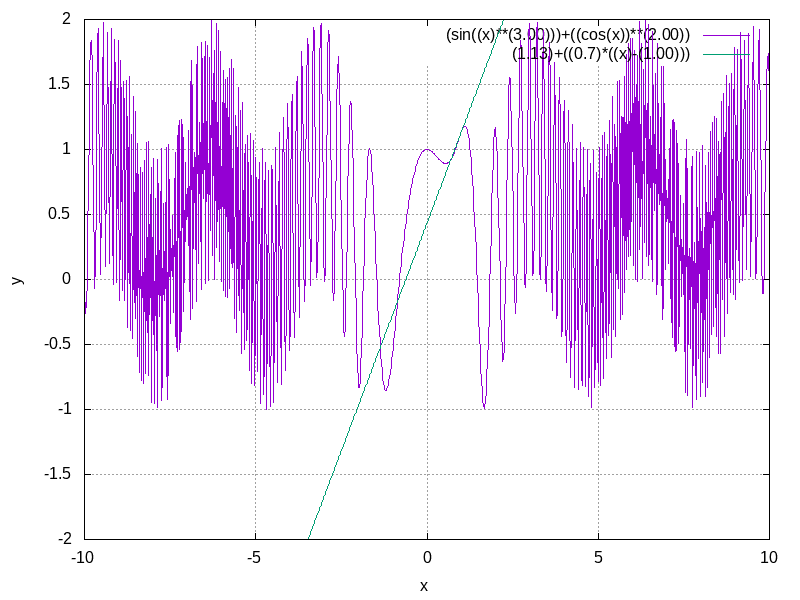
\includegraphics[width=0.8\linewidth]{func.png}
\caption{график функций полученный после комплексного анализа}
\label{fig:mpr}
\end{figure}
\end {document}